\documentclass[11pt,a4paper]{article}
\usepackage[margin=23mm]{geometry}
\usepackage{amsmath,booktabs,graphicx,siunitx,hyperref}
\title{CSA compression in complete ion-pad histories}
\date{\today}
\begin{document}\maketitle
\section{Calculation and coverage}
The stored uncut counts supply complete pad histories for 8000 double-beta and
8000 electron events. The same diffused events are studied at 2 mm pitch with
20 ms buckets and 4 mm pitch with 40 ms buckets. Every missing sparse entry is
filled with zero. Each event starts at the quiescent CSA operating point.

The optimized 180 nm CSA uses a grounded $M_f$ gate, $M_f$ width 0.36 $\mu$m and
length 400 $\mu$m, $M_4$ gate 0.6164 V, $C_f=3$ fF and external input
capacitance 1.25 pF. The input current uses uniform collection times within each
bucket and the on-axis square-pad benchmark: side 0.5 mm, grounded surrounding
plane, 5 mm final gap and constant speed 3 m/s. Its integral is
$e[1-\phi_w(g)]$ per ion. The fixed-geometry weighting potential uses a unit pad
and zero surrounding plane. This calculation remains the planar benchmark for
the final approach.

All histories whose minimum linear voltage is below 0.35 V are run directly
in LTspice. Each sample also supplies twelve fixed-seed control histories in
each of the four higher-voltage ranges: 0.35--0.5, 0.5--0.65, 0.65--0.8 and
0.8--1 V. The latter upper edge covers the 0.884 V baseline. The three-second
post-event tail preserves the discharge after collection.

\begin{table}[ht]\centering
\begin{tabular}{lrrr}\toprule
Sample & Candidate pads & Controls & Refined histories\\\midrule
2 mm / 20 ms, $0\nu\beta\beta$ & 9 & 48 & 1 \\
2 mm / 20 ms, electrons & 5 & 48 & 1 \\
4 mm / 40 ms, $0\nu\beta\beta$ & 2236 & 48 & 17 \\
4 mm / 40 ms, electrons & 1488 & 48 & 6 \\
\bottomrule\end{tabular}
\caption{Completed transistor simulations. Each source contains 8000 events.}
\end{table}

Voltages are averaged over 5 ms centred at frame boundaries. Both the linear
and transistor responses use the same corrected difference,
$D_n=-[\Delta\overline V_n-\alpha\Delta\overline V_{n-1}]$, with
$\alpha=\exp(-\Delta t/\tau)$. The fixed low-charge gain $g$ expresses the
frame estimate as $D_n/g$. Responses include current before collection and
spreading from the averaging windows.

\section{Response-loss criteria}
For each bucket with collected ions, the relative response loss and missing
signal are
\begin{equation}
 L_n=\max\!\left(0,1-\frac{D_n^{\mathrm{SPICE}}}{D_n^{\mathrm{linear}}}\right),\qquad
 d_n=\frac{\max(0,D_n^{\mathrm{linear}}-D_n^{\mathrm{SPICE}})}{g}.
\end{equation}
A bucket is flagged when $L_n$ exceeds the chosen fractional loss and $d_n$
exceeds a selected multiple of the nominal quiescent ENC. An event is counted
once when any tested pad contains such a bucket. All collected inputs are
retained. The zero, one and three ENC criteria are saved; the tables below use
one ENC as the minimum missing signal. This scale refers to a deficit in the
mean response. Random electronic noise is not added to these transients.

\begin{table}[ht]\centering
\begin{tabular}{lrrrr}\toprule
Sample & Loss $\geq10\%$ & $\geq25\%$ & $\geq50\%$ & $\geq75\%$\\\midrule
2 mm / 20 ms, $0\nu\beta\beta$ & 0.11 & 0.06 & 0.01 & 0.00 \\
2 mm / 20 ms, electrons & 0.05 & 0.01 & 0.01 & 0.00 \\
4 mm / 40 ms, $0\nu\beta\beta$ & 19.19 & 11.19 & 5.94 & 1.86 \\
4 mm / 40 ms, electrons & 13.03 & 7.74 & 4.29 & 1.32 \\
\bottomrule\end{tabular}
\caption{Percentage of all 8000 events with confirmed response loss in at least
one occupied bucket, with a deficit of at least one nominal ENC.}
\end{table}
\begin{figure}[ht]\centering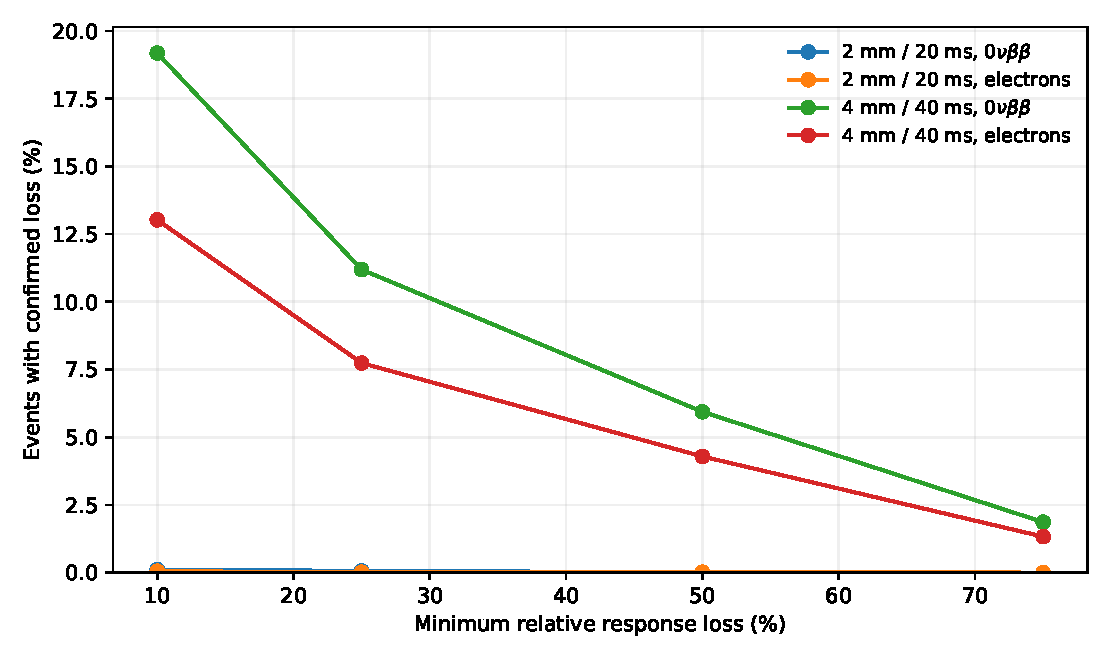
\includegraphics[width=.95\linewidth]{event_fractions.pdf}
\caption{Event fractions versus compression severity for the one-ENC deficit criterion.}
\end{figure}

These are confirmed rates within the configured candidate and control study.
The control sample checks the screening range; it does not supply an exhaustive
measurement of every unsimulated pad. The quoted criterion concerns a local
response loss. Whether a flagged event remains useful is assessed by track
reconstruction with the affected locations retained.

\section{How much of an event is affected?}
The affected-ion fraction sums the collected ions in flagged buckets and divides
by the full collected ion count of that event. For the 50\% loss and one-ENC
deficit criterion, its distribution among flagged events is:
\begin{table}[ht]\centering
\begin{tabular}{lrrr}\toprule
Sample & Median (\%) & 90th percentile (\%) & Maximum (\%)\\\midrule
2 mm / 20 ms, $0\nu\beta\beta$ & 0.20 & 0.20 & 0.20 \\
2 mm / 20 ms, electrons & 0.77 & 0.77 & 0.77 \\
4 mm / 40 ms, $0\nu\beta\beta$ & 1.38 & 5.82 & 19.99 \\
4 mm / 40 ms, electrons & 1.11 & 5.37 & 16.12 \\
\bottomrule\end{tabular}
\caption{Fraction of event ions located in buckets satisfying the severe-loss criterion.}
\end{table}
\begin{figure}[ht]\centering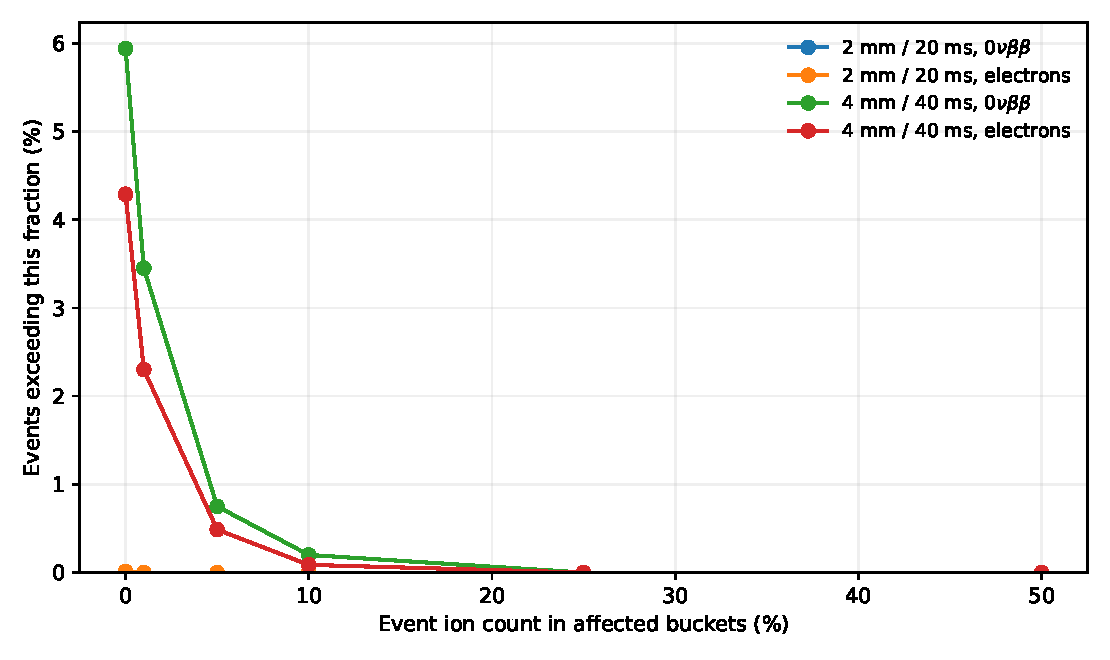
\includegraphics[width=.95\linewidth]{affected_charge.pdf}
\caption{Fraction of all events exceeding a given affected-ion fraction, using
50\% response loss and at least one ENC of missing signal.}
\end{figure}
This observable locates charge in affected buckets. The saved positive deficit
in frame estimates provides a separate measure of the signal reduction.

\section{Controls and validation}
\begin{table}[ht]\centering\small
\begin{tabular}{lrrrr}\toprule
Sample & 0.35--0.5 V & 0.5--0.65 V & 0.65--0.8 V & 0.8--1 V\\\midrule
2 mm / 20 ms, $0\nu\beta\beta$ & 7.76 & 8.09 & 3.30 & 0.27 \\
2 mm / 20 ms, electrons & 10.05 & 10.29 & 2.65 & 0.21 \\
4 mm / 40 ms, $0\nu\beta\beta$ & 39.26 & 11.91 & 2.26 & 0.21 \\
4 mm / 40 ms, electrons & 66.96 & 70.75 & 13.51 & 0.31 \\
\bottomrule\end{tabular}
\caption{Largest relative loss (\%) among twelve controls in each stratum,
including small deficits. The stored flag counts also apply the ENC criterion.}
\end{table}
The numbers of sampled controls with both at least 10\% response loss and one
ENC missing signal are 0, 0, 0, 0, in the table order. Large relative losses
in a very small signal can therefore be distinguished from an appreciable
missing response.

Input PWL integrals preserve the finite-path charge to relative error below
$10^{-8}$. Every accepted SPICE transient passes a sampled-current charge check
at $10^{-7}$. A failed exported-current check triggers smaller solver steps.
The no-input waveform agrees with the saved operating-point baseline to below
$10^{-9}$ V. Refined histories halve the current-knot and solver steps; the
largest normalized change of frame signal is \num{2.490e-06}.

Julia validates completed study coverage, nested response-loss criteria, event
counting, affected charge bounds and resolution convergence. The viewer
integration checks compare source counts, zero-bucket restoration, the earlier
matched-baseline SPICE calculation and the live HTTP interface.

\section{Viewer and reproduction}
\begin{verbatim}
python scripts/viewers/view_pad_histories.py
python scripts/electronics/histories/run_pad_compression.py --workers 4
\end{verbatim}
The viewer provides event and pad selection, linked plots of collected counts,
CSA voltage and frame estimates, on-demand cached SPICE simulations, and the
compression table. The batch acquires missing candidate/control simulations and
saves event statistics. Julia reduction and report presentation are also
available separately:
\begin{verbatim}
julia --project=. scripts/electronics/histories/report_pad_compression.jl RESULTS_DIRECTORY
python scripts/electronics/histories/present_pad_compression.py --results RESULTS_DIRECTORY
\end{verbatim}
Results are stored in \texttt{results/ltspice/pad\_compression/caac67eddc10/}.
Their provenance records source-screen, physical-code, calibration, model and
configuration hashes. Each case records its simulator and netlist hashes.
The report source is generated without compiling a PDF.
\end{document}
